%% fig_nsem_workflow.tex -- standalone TikZ source for Figure 2 of
%% "Sparse data limit what a corrosion model can predict".
%%
%% One workflow: how the reduced point defect model is inverted from the
%% three exposure times by physics-informed training on a spectral-element
%% node set, and how the identified kinetics are graded against the exact
%% closed-form solution before they are used.
%%
%% Build:  pdflatex fig_nsem_workflow.tex
%% (scripts/make_fig_nsem_workflow.sh also rasterizes it to .png)

\documentclass[tikz,border=6pt]{standalone}
\usepackage{amsmath,amssymb}
\usepackage{helvet}
\renewcommand{\familydefault}{\sfdefault}
\usepackage{sansmath}
\usetikzlibrary{arrows.meta,positioning,shapes.geometric,calc,fit,backgrounds}

\begin{document}\sansmath
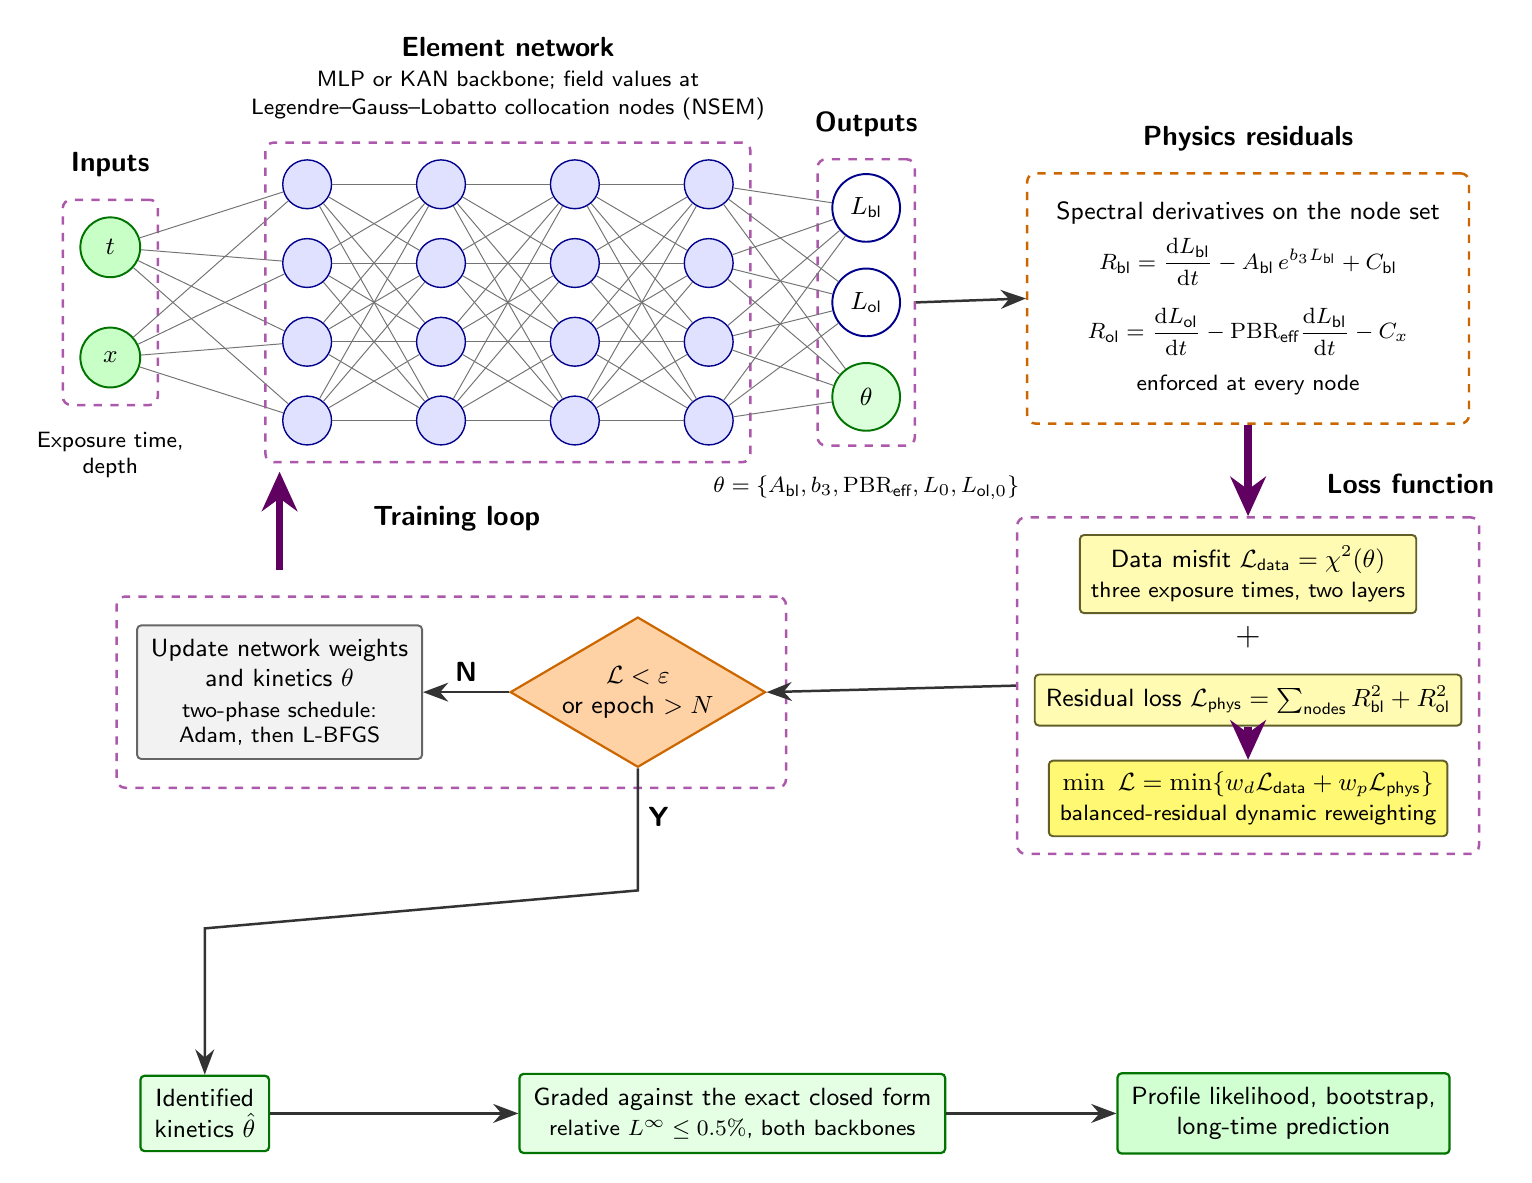
\begin{tikzpicture}[
  font=\sffamily\small,
  >={Stealth[length=3.2mm,width=2.4mm]},
  neuron/.style={circle,draw=blue!55!black,fill=blue!12,minimum size=6.2mm,inner sep=0pt,line width=0.5pt},
  innode/.style={circle,draw=green!45!black,fill=green!22,minimum size=7.6mm,inner sep=0pt,line width=0.7pt},
  outnode/.style={circle,draw=blue!55!black,fill=white,minimum size=8.6mm,inner sep=0pt,line width=0.7pt},
  panel/.style={rounded corners=3pt,draw=violet!65,dashed,line width=0.9pt},
  physpanel/.style={rounded corners=3pt,draw=orange!80!black,dashed,line width=0.9pt},
  lbox/.style={rectangle,rounded corners=1.5pt,draw=olive!60!black,fill=yellow!30,
               line width=0.7pt,align=center,inner sep=4pt},
  tbox/.style={rectangle,rounded corners=1.5pt,draw=black!60,fill=black!5,
               line width=0.7pt,align=center,inner sep=5pt},
  obox/.style={rectangle,rounded corners=1.5pt,draw=green!45!black,fill=green!10,
               line width=0.8pt,align=center,inner sep=5pt},
  dia/.style={diamond,aspect=1.7,draw=orange!80!black,fill=orange!35,line width=0.8pt,
              align=center,inner sep=1pt},
  title/.style={font=\sffamily\bfseries},
  link/.style={draw=black!55,line width=0.35pt},
  flow/.style={->,line width=0.9pt,draw=black!80},
  fat/.style={-{Stealth[length=5mm,width=4.5mm]},line width=2.6pt,draw=violet!75!black},
]

%% ---------------------------------------------------------------- inputs
\node[innode] (in1) at (1.40,13.20) {$t$};
\node[innode] (in2) at (1.40,11.80) {$x$};
\node[panel,fit=(in1)(in2),inner sep=6pt] (inbox) {};
\node[font=\sffamily\footnotesize,align=center,below=2mm of inbox]
  {Exposure time,\\ depth};
\node[title,above=1.5mm of inbox] {Inputs};

%% --------------------------------------------------------------- network
\foreach \lx [count=\li] in {3.90,5.60,7.30,9.00}{
  \foreach \ly [count=\lj] in {14.00,13.00,12.00,11.00}{
    \node[neuron] (h\li-\lj) at (\lx,\ly) {};
  }
}
\foreach \li/\lk in {1/2,2/3,3/4}{
  \foreach \lj in {1,...,4}{ \foreach \lm in {1,...,4}{
    \draw[link] (h\li-\lj) -- (h\lk-\lm);
  }}
}
\foreach \lj in {1,...,4}{
  \draw[link] (in1) -- (h1-\lj);
  \draw[link] (in2) -- (h1-\lj);
}
\node[panel,fit=(h1-1)(h4-4),inner sep=6pt] (netbox) {};
\node[title,above=1.5mm of netbox,align=center]
  {Element network\\[-1pt] \footnotesize\mdseries MLP or KAN backbone; field values at\\[-2pt]
   \footnotesize\mdseries Legendre--Gauss--Lobatto collocation nodes (NSEM)};

%% ---------------------------------------------------------------- output
\node[outnode] (o1) at (11.00,13.70) {$L_\text{bl}$};
\node[outnode] (o2) at (11.00,12.50) {$L_\text{ol}$};
\node[outnode,draw=green!45!black,fill=green!14] (o3) at (11.00,11.30) {$\theta$};
\node[panel,fit=(o1)(o2)(o3),inner sep=5pt] (outbox) {};
\node[title,above=1.5mm of outbox] {Outputs};
\foreach \lj in {1,...,4}{
  \draw[link] (h4-\lj) -- (o1);
  \draw[link] (h4-\lj) -- (o2);
  \draw[link] (h4-\lj) -- (o3);
}
\node[font=\sffamily\footnotesize,align=center] at (11.00,10.15)
  {$\theta=\{A_\text{bl},b_3,\mathrm{PBR}_\text{eff},L_0,L_{\text{ol},0}\}$};

%% -------------------------------------------------------------- physics
\node[align=center,font=\sffamily\footnotesize] (phys) at (15.85,12.55)
  {\small Spectral derivatives on the node set\\[4pt]
   $\displaystyle R_\text{bl}=\frac{\mathrm{d}L_\text{bl}}{\mathrm{d}t}
      -A_\text{bl}\,e^{b_3 L_\text{bl}}+C_\text{bl}$\\[7pt]
   $\displaystyle R_\text{ol}=\frac{\mathrm{d}L_\text{ol}}{\mathrm{d}t}
      -\mathrm{PBR}_\text{eff}\frac{\mathrm{d}L_\text{bl}}{\mathrm{d}t}-C_x$\\[6pt]
   enforced at every node};
\node[physpanel,fit=(phys),inner sep=7pt] (physbox) {};
\node[title,above=1.5mm of physbox] {Physics residuals};
\draw[flow] (outbox.east) -- (physbox.west);

%% ------------------------------------------------------------------ loss
\node[lbox] (ldata) at (15.85,9.05)
  {Data misfit $\mathcal{L}_\text{data}=\chi^2(\theta)$\\
   \footnotesize three exposure times, two layers};
\node[font=\sffamily\large\bfseries] (plus) at (15.85,8.25) {$+$};
\node[lbox] (lphys) at (15.85,7.45)
  {Residual loss $\mathcal{L}_\text{phys}=\sum_\text{nodes}R_\text{bl}^2+R_\text{ol}^2$};
\node[lbox,fill=yellow!55] (ltot) at (15.85,6.20)
  {$\min\ \mathcal{L}=\min\{w_d\mathcal{L}_\text{data}+w_p\mathcal{L}_\text{phys}\}$\\
   \footnotesize balanced-residual dynamic reweighting};
\draw[fat] (lphys) -- (ltot);
\node[panel,fit=(ldata)(lphys)(ltot),inner sep=6pt] (lossbox) {};
\node[title,anchor=east] at (19.10,10.20) {Loss function};
\draw[fat] (physbox.south) -- (lossbox.north);

%% --------------------------------------------------------- training loop
\node[dia] (conv) at (8.10,7.55) {$\mathcal{L}<\varepsilon$\\ or epoch $>N$};
\node[tbox] (upd) at (3.55,7.55)
  {Update network weights\\ and kinetics $\theta$\\
   \footnotesize two-phase schedule:\\[-2pt] \footnotesize Adam, then L-BFGS};
\node[panel,fit=(conv)(upd),inner sep=7pt] (loopbox) {};
\node[title] at (5.80,9.75) {Training loop};
\draw[flow] (lossbox.west) -- (conv.east);
\draw[flow] (conv.west) -- node[above,font=\sffamily\bfseries]{N} (upd.east);
\draw[fat] (3.55,9.10) -- (3.55,10.35);

%% -------------------------------------------------------------- outcomes
\node[obox] (oth) at (2.60,2.20) {Identified\\ kinetics $\hat\theta$};
\node[obox] (over) at (9.30,2.20)
  {Graded against the exact closed form\\
   \footnotesize relative $L^\infty\le0.5\%$, both backbones};
\node[obox,fill=green!18] (odown) at (16.30,2.20)
  {Profile likelihood, bootstrap,\\ long-time prediction};
\draw[flow] (oth) -- (over);
\draw[flow] (over) -- (odown);
\draw[flow] (conv.south) -- node[right,pos=0.4,font=\sffamily\bfseries]{Y} ++(0,-1.55)
  -- (2.60,4.55) -- (oth.north);

\end{tikzpicture}
\end{document}
